\documentclass[letterpaper,journal]{IEEEtran}

\usepackage{amsmath,amsfonts}
\usepackage{graphicx}
\usepackage{cite}

\begin{document}

\title{Contact-Aware Retargeting Network}
\author{} % Add author names and affiliations when available.

\maketitle

\begin{abstract}
We introduce the Contact-Aware Retargeting Network (CART), a neural method for transferring human manipulation from a tactile glove to a dexterous robot hand. Geometric retargeting can preserve finger motion while losing task-relevant contacts when human and robot hands differ in size, proportions, and kinematics. Some existing methods reconstruct the scene and then use reinforcement learning to train task-specific manipulation policies, a process that requires scene setup and policy tuning. CART extracts contact anchors from active tactile sensors for training and uses cross-attention to fuse tactile observations with five fingertip poses over a buffered ten-frame window. Conditioned on the current robot configuration, five finger-specific decoders predict joint increments from a shared representation. Differentiable contact and collision objectives guide training, and a forward pass predicts each update without iterative optimization. The same formulation targets both prehensile and nonprehensile manipulation.
\end{abstract}

\begin{IEEEkeywords}
Egocentric Data, Dexterous Manipulation, Motion Retargeting, Tactile Sensing.
\end{IEEEkeywords}

% !TeX root = main.tex
\section{Introduction}
\label{sec:introduction}

\IEEEPARstart{D}{exterous} manipulation is central to everyday human activity. Vision--language--action (VLA) models are beginning to address manipulation with dexterous hands~\cite{wen2025dexvla}, creating demand for demonstrations that capture the contact patterns of human-like five-finger hands. For many parallel-jaw grasps, adjusting the gripper aperture is enough to close an unintended gap. A five-finger hand can contact an object with different combinations of fingertips, finger links, and palm regions. Retargeting must account for which regions make contact as well as how the fingers move. Even efficient kinematic methods can leave task-relevant contacts unrealized, making both teleoperation and the conversion of egocentric demonstrations into reliable robot actions more difficult.

Transferring a manipulation skill across embodiments poses two coupled problems: identifying the contact anchors that matter for the task and adapting the robot's posture to realize them. Differences in hand size, shape, and kinematics make exact alignment of all human keypoints generally infeasible. A pose objective that treats all keypoints alike can sacrifice a contact needed to execute the task. The relevant anchors also change across skills and over the course of a demonstration.
% Add Fig.~\ref{fig:contact-anchors} here once the CART contact-anchor figure is available.
Preserving these anchors may require shifting the contact to a different point on the corresponding robot surface and allowing some deviation from the demonstrated posture. We therefore prioritize the contacts needed to reproduce the skill.

Kinematic retargeting methods such as DexPilot, AnyTeleop, and GeoRT efficiently map human hand motion to robot configurations~\cite{handa2019dexpilot,qin2023anyteleop,yin2025geort}, but their kinematic objectives cannot ensure that the robot makes the intended contact with the object. Some methods import object meshes into a simulator and use reinforcement learning to reproduce manipulation skills~\cite{mandi2025dexmachina}. Building and tuning task-specific environments makes this approach difficult to scale across demonstrations, and object meshes are privileged information that may be unavailable during real-world operation. TouchBridge and CARD use contact information, including tactile measurements, to guide retargeting~\cite{zhang2026touchbridge,dai2026card}. Their results show the value of preserving demonstrated contacts, and tactile measurements provide a common representation across tasks without object models. Both frameworks use optimization to produce retargeted trajectories for offline data processing or replay. They address embodiment differences through contact alignment or semantic correspondences, leaving open how to predict robot-specific posture adjustments directly from a sequence of tactile observations.

We propose the Contact-Aware Retargeting Network (CART) for transferring manipulation from tactile gloves to five-finger robot hands. CART conditions on the current robot configuration and uses cross-attention to fuse a short sequence of human fingertip poses and tactile signals. It predicts joint increments that promote contact preservation and temporal smoothness. A forward pass produces each update, supporting offline processing and buffered online retargeting.

The contributions of this paper are summarized as follows:
\begin{enumerate}
    \item We introduce a contact-aware retargeting network that uses a shared pose and tactile representation and five finger-specific decoders to transfer manipulation skills without object geometry or pose observations.
    \item We develop a training pipeline covering hand calibration, glove data collection, differentiable objective design, and policy training. In our setup, training uses about 5~min of recorded glove data and takes approximately 3~GPU-hours on a single NVIDIA A800.
    \item We develop an arm retargeting procedure that adjusts the end-effector target pose using contact anchors and computes arm motion through efficient inverse kinematics.
    % Add the corresponding task list, baseline results, and timing breakdown in Section~\ref{sec:experiments}.
    \item We evaluate CART on prehensile and nonprehensile manipulation tasks, including in-hand manipulation. In these comparisons, CART maintains contact more reliably and produces smoother trajectories, with shorter inference times relative to the evaluated baselines.
\end{enumerate}

% !TeX root = main.tex
\section{Related Work}
\label{sec:related}

\subsection{Kinematic Retargeting}
Kinematic retargeting maps human hand motion to robot configurations by preserving geometric features such as finger directions and fingertip positions. DexPilot, AnyTeleop, wuji-retargeting, and GeoRT support low-latency hand retargeting for teleoperation~\cite{handa2019dexpilot,qin2023anyteleop,wuji2026retargeting,yin2025geort}. GeoRT maps fingertip positions directly through a neural model, and the public wuji-retargeting interface takes wrist-relative hand landmarks. Both include pinch-specific objectives or target adjustments. These mechanisms encourage fingertip closure in selected poses, but the hand geometry alone leaves object contacts unspecified. Consequently, a visually similar posture can lose the distributed contacts needed to grasp a large object or the sustained surface contact needed for nonprehensile manipulation.

\subsection{Object-Aware Retargeting}
Contact-aware methods can trade some pose-tracking accuracy for more stable task-relevant contacts. OATH rolls out a shared residual reinforcement learning policy in simulation, using contact errors relative to the object surface to refine a kinematic reference~\cite{sigurdson2026oath}. C2Dex aggregates stable contacts in the object's canonical frame, preserves local hand--object geometry during retargeting, and applies residual reinforcement learning in simulation~\cite{ren2026c2dex}. Do as I Do reconstructs hand and object motion from monocular video and searches for feasible robot trajectories with sampling-based model predictive control~\cite{paliwal2026doasido}. DexForge uses spherical-Gaussian object models in a differentiable simulator and refines contact-aware kinematic references through gradient-based, force-aware control optimization~\cite{wang2026dexforge}. Generative Neural Retargeting (GNR) uses flow matching to sample control corrections and aims to generalize across objects and demonstrations~\cite{gao2026gnr}. Its retargeting pipeline still requires object surface geometry and per-frame object poses, which must be estimated when they are unavailable from motion capture. These methods rely on object geometry and demonstrated or reconstructed object states during retargeting. When such information is recovered from video, occlusions can degrade pose estimates, and geometric reconstruction errors can shift predicted contacts. The need for object information during retargeting is distinct from whether the resulting trajectory is executed with object-state feedback.

\subsection{Tactile Retargeting}
Tactile measurements provide direct evidence of which hand regions touch an object without requiring an explicit object model. TouchBridge aligns fingertip contact-patch centers and active taxels, preserves their spatial relationships, and relaxes fingertip pose tracking when contact is detected~\cite{zhang2026touchbridge}. Its contact representation is limited to the sensor patches on the fingertips. CARD defines contact-force targets across hand regions, including the fingers and palm, and uses per-frame GPU sampling to solve for robot configurations~\cite{dai2026card}. It computes retargeted trajectories offline and uses tactile feedback to track force targets during hardware replay. CART uses a learned mapping from glove tactile observations and fingertip poses to support both offline data conversion and buffered online retargeting.

% !TeX root = main.tex
\section{Method}
\label{sec:method}

CART transfers finger motion from a tactile glove to the 20-DoF Wuji2 hand. The policy predicts a sequence of joint updates from measured glove signals. During training, a calibrated human hand mesh provides geometric targets, and differentiable robot geometry maps contact and collision errors to joint-space gradients (Fig.~\ref{fig:cart-overview}).

\begin{figure*}[t]
    \centering
    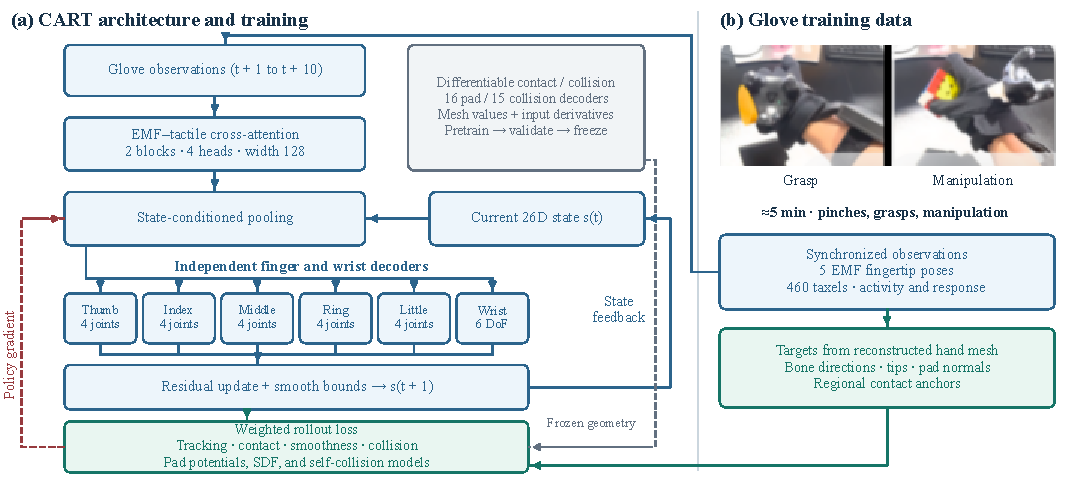
\includegraphics[width=\textwidth]{figs/cart_overview.pdf}
    \caption{CART architecture and training data. Left, five finger-specific decoders share an observation encoder. Weighted tracking, contact, smoothness, and collision losses backpropagate through the predicted states. Detached predictions provide native-mesh supervision for separate geometry updates. Right, synchronized glove signals and derived training targets. The photographs illustrate tactile-glove acquisition.}
    \label{fig:cart-overview}
\end{figure*}

\subsection{Network Architecture}
\label{sec:cart-architecture}

At step $t$, the policy receives the current robot joint angles $q_t$ and a window of ten measured glove frames, from $t+1$ through $t+10$. Each frame contains the electromagnetic (EMF) receiver pose for each of the five fingertips and the positions and binary contact states of 460 tactile elements (taxels). We express spatial observations in a canonical hand frame and represent each receiver rotation by its first two matrix columns. Relative timestamps encode the interval from the current robot state, and validity masks mark missing measurements. Online inference buffers the measured lookahead window before producing an update.

The encoder projects EMF and tactile inputs into 128-dimensional tokens and adds embeddings for frame index, relative time, and finger or taxel identity. Two four-head cross-attention blocks use the EMF tokens as queries and the tactile tokens as keys and values. Each head uses scaled dot-product attention with a mask for invalid keys. Each block applies residual connections around attention and its feed-forward layer. A further attention block uses an embedding of the current normalized joint state to pool the fused tokens into a shared representation. Five independent multilayer perceptrons, each with two 256-unit hidden layers, decode this representation into four joint increments per finger. Let $z_t$ denote the pooled context and $D_f$ the decoder for finger $f$. The normalized increment $\Delta\bar q_t$ concatenates the five outputs $D_f(z_t)$ in thumb-to-little-finger order. A $\tanh$ output bounds each increment. Let $\bar q$ denote joint angles rescaled to $[-1,1]$ using the robot's joint limits. The next state is given by
\begin{equation}
    \bar q_{t+1} = \operatorname{clip}
    \bigl(\bar q_t + \Delta\bar q_t,\,-1,\,1\bigr).
    \label{eq:cart-state-update}
\end{equation}
For joint $j$ with limits $(l_j,u_j)$, normalization uses $\bar q_{t,j}=2(q_{t,j}-l_j)/(u_j-l_j)-1$. Thus a decoder output has the same normalized range across joints, while its physical scale depends on the joint range. We map the clipped state back to radians for forward kinematics and feed it into the next update. The shared encoder lets a finger's decoder use observations from the other fingers.

\subsection{Hand Mesh Estimation}
\label{sec:cart-hand-mesh}

We reconstruct the demonstrator's hand using a skinned template driven by an articulated hand model. Six calibration poses comprise four thumb-to-finger pinches, a pose with the four finger bases flexed and the remaining joints extended, and a flat palm. We jointly fit finger bone lengths, the rigid receiver-to-distal-link transforms, and the transmitter-to-wrist transform. We compose the transmitter-to-wrist alignment, distal-link forward kinematics, and receiver mounting transform to predict each receiver pose in the transmitter frame. The fit uses measured EMF positions and orientations, contact and posture constraints from the calibration poses, and regularization on the fitted parameters. With these parameters fixed, we estimate hand joint angles frame by frame using joint-bounded inverse kinematics on the measured EMF poses.

Linear blend skinning deforms the template with the estimated joint angles. Each taxel is attached to a mesh triangle by fixed barycentric coordinates, so its position is $x_i=\sum_{k=1}^{3}\beta_{ik}v_{ik}$, where $\beta_{ik}$ are fixed weights and $v_{ik}$ are the deformed triangle vertices. Let $\mathcal I_r$ index active taxels in region $r$ and let $s_i$ denote tactile response. The operator $\Pi$ projects the response-weighted center of pressure onto the observed surface triangles $\mathcal S_r$,
\begin{equation}
    a_r=\Pi_{\mathcal S_r}\!\left(
        \frac{\sum_{i\in\mathcal I_r}s_i x_i}{\sum_{i\in\mathcal I_r}s_i}
        \right).
    \label{eq:cart-anchor}
\end{equation}
The projected point $a_r$ and response-weighted surface normal $n_r$ supervise the corresponding robot region. The encoder receives binary contact states, while the contact targets retain the tactile response.

\subsection{Training Framework}
\label{sec:cart-training}

\textit{Data and rollout.} We record approximately 5~min of glove data covering free-form finger pinches, grasps, and object manipulation. The recordings provide synchronized fingertip poses and tactile observations, from which we compute geometric and contact targets. We train on contiguous windows, using inverse kinematics to initialize the robot hand at the first frame. The policy then rolls out 16 updates per window, feeding back its own predicted joint state at each step. A transition from $q_t$ to $q_{t+1}$ uses its own ten-frame buffer and is scored against targets at $t+1$. The other frames provide measurement context for that transition. Because the observation encoder is independent of $q_t$, its outputs can be computed in parallel across the rollout. The joint-conditioned pooling and decoding then run sequentially, preserving the dependence on the predicted state.

\textit{Differentiable geometry and objective.} The policy transition, forward kinematics, and tracking and contact terms are differentiable with respect to the predicted joints almost everywhere. Joint-limit clipping and the tactile-depth maximum are piecewise differentiable. Contact alignment uses a learned pad projector. Native self-collision queries require discrete closest-feature selection, so we handle self-collision with a differentiable surrogate. Robot forward kinematics supplies link poses for bone-direction, fingertip-position, and distal-pad-normal tracking. For active region $r$, let $(R_r(q),p_r(q))$ be the pose of its robot link. We transform the anchor $a_r$ from~\eqref{eq:cart-anchor} into link coordinates as $x_r=R_r^\top(a_r-p_r)$. The projection may bias this query toward the demonstrated longitudinal position on the pad. Given the resulting query, the learned projector predicts a local point $y_r$ and unit normal $m_r$. We express them in the wrist frame as $\hat a_r=R_r y_r+p_r$ and $\hat n_r=R_r m_r$. The link pose affects both the query and the projected result. The alignment cost weights the position and normal errors over active regions as specified in Table~\ref{tab:cart-loss}. The response multiplier $\rho_r=1+0.5F_r/\max_j F_j$ uses the regional response $F_r$ relative to the strongest response in the frame, with a positive denominator floor. For regions active in consecutive frames, the objective penalizes displacement of the projected point in link coordinates and the gap between the current anchor and the corresponding pad surface. The cost also includes a squared joint displacement term.

An articulated neural signed-distance field (SDF) evaluates active glove points against specified robot links. Even with differentiable per-link SDFs, a closest-link formulation of self-collision requires selecting a link pair. The selected pair can change as the joints move, and the minimum-distance gradient can switch at ties. We instead train a smooth network that takes only $q$ and predicts self-clearance energy $\widehat E_{\rm self}$, maximum penetration depth $\widehat d_{\max}$, and the norm $\widehat D$ of sampled penetrations. A smooth threshold of the predicted depth gives a collision score, and the gradient of the weighted clearance and penetration costs gives a joint-space direction for reducing collision. Native geometry queries generate training labels for the values, joint derivatives, and escape direction. The policy graph evaluates the learned self-collision model directly from $q$.

Table~\ref{tab:cart-loss} specifies the per-step terms and weights. Distance residuals use millimeters, joint differences use radians, and directional errors use $1-u^\top v$ for unit vectors. For self-clearance, the teacher sums squared violations of a 6~mm margin across sampled points. For tactile penetration, the neural SDF supplies signed distances $s_k$ to the queried links, with $d_{\rm touch}=\max_k[-s_k]_+$ and $[x]_+=\max(0,x)$. The 5~mm guard applies separately to the predicted self-penetration norm and the maximum tactile penetration.

\begin{table}[t]
\caption{Per-step residuals and loss coefficients}
\label{tab:cart-loss}
\centering
\small
\begin{tabular}{@{}llr@{}}
\hline
Term & Residual $\ell_k$ & $\lambda_k$ \\
\hline
Bone direction & Sum of directional errors & $20^2$ \\
Fingertip position & Sum of squared distances & $3^2$ \\
Distal-pad normal & Sum of directional errors & $60^2$ \\
Joint smoothness & $\|q_t-q_{t-1}\|_2^2$ & $0.1^2$ \\
Contact position & $\sum_r \rho_r^2\|\hat a_r-a_r\|_2^2$ & $40^2$ \\
Contact normal & $\sum_r \rho_r^2(1-\hat n_r^\top n_r)$ & $40^2\cdot2\cdot10^2$ \\
Material continuity & Link-local drift squared & $2.5^2$ \\
Link continuity & Anchor-to-pad gap squared & $2.5^2$ \\
Self-clearance & $\widehat E_{\rm self}(q_t)$ & $1.5^2$ \\
Tactile penetration & $\sum_k[-s_k-2]_+^2$ & $3.5^2$ \\
Penetration guard & $[\widehat D-5]_+^2+[d_{\rm touch}-5]_+^2$ & $40^2$ \\
\hline
\end{tabular}
\end{table}

The two continuity residuals sum over regions active across both frames, with each squared error multiplied by $\rho_r^2$. When a frame has no tactile queries, its tactile penetration residual and $d_{\rm touch}$ are zero. At each predicted state, the weighted cost is $c_{b,t}=\sum_k\lambda_k\ell_{k,b,t}$. For $N$ windows of 16 steps each, the normalized batch loss is
\begin{equation}
    \mathcal L=\frac{C}{C+10^6},\qquad
    C=\frac{1}{16N}\sum_{b,t}c_{b,t}.
    \label{eq:cart-training-loss}
\end{equation}

\textit{Backpropagation through time.} Write~\eqref{eq:cart-state-update} as $\bar q_{t+1}=F_\theta(\bar q_t,o_t)$, with buffered observations $o_t$ and policy parameters $\theta$. With state sensitivity $S_t=\mathrm d\bar q_t/\mathrm d\theta$ and fixed initialization $S_0=0$, the recurrence is
\begin{equation}
    S_{t+1}=\frac{\partial F_\theta}{\partial\theta}
       +\frac{\partial F_\theta}{\partial\bar q_t}S_t.
    \label{eq:cart-bptt}
\end{equation}
Reverse-mode backpropagation through time (BPTT) evaluates~\eqref{eq:cart-bptt} across all 16 updates. Thus later contact and collision losses contribute to the gradient of earlier predictions. The continuity terms also depend directly on consecutive configurations. Joint-limit clipping is piecewise differentiable and preserves the residual state path in the interior of the joint bounds. We truncate gradients at window boundaries.

For each batch, we retain the policy rollout graph and detach a copy of the predicted states to generate native-mesh labels. We take two geometry optimizer steps and then freeze the geometry parameters when evaluating~\eqref{eq:cart-training-loss} on the retained rollout. Gradients still flow through the frozen models into the joint state and through geometry queries that depend on the moving links. One BPTT update then trains the shared encoder and all five decoders using contact gradients evaluated at configurations visited by the current policy.

\subsection{Arm Motion Retargeting}
\label{sec:cart-arm}

We express the demonstrated contact anchors in the virtual reality (VR) world frame. Given the finger configuration predicted by CART, robot hand forward kinematics gives the corresponding contact locations relative to the robot wrist. We place the wrist in the VR world so that these locations align with the demonstrated anchors, using the tracked human wrist pose as a reference when the anchors underconstrain the pose.

We fit a single rigid transform \({}^{V}T_B\) from the robot base frame $B$ to the VR world frame $V$. For calibration sample $i$, let $(R_i^B,p_i^B)$ be the wrist pose obtained from arm forward kinematics and $(R_i^V,p_i^V)$ the paired wrist target in VR. The position residual is $e_i=Rp_i^B+p-p_i^V$ and the orientation residual is $E_i=RR_i^B-R_i^V$. We solve the weighted least-squares problem
\begin{equation}
    (R^*,p^*)=\arg\min_{R,p}\sum_i
        \left(\|e_i\|_2^2+\lambda_R\|E_i\|_F^2\right).
    \label{eq:cart-vr-base}
\end{equation}
Here $R\in SO(3)$, $p\in\mathbb R^3$, and $\lambda_R$ balances translation and rotation. The fit in~\eqref{eq:cart-vr-base} yields \({}^{V}T_B=(R^*,p^*)\). We convert each VR wrist target to the robot base frame as \({}^{B}T_{W,t}=({}^{V}T_B)^{-1}{}^{V}T_{W,t}\). The arm inverse kinematics solver tracks this target using the previous arm configuration as its initial guess.

% !TeX root = main.tex
\section{Experiments}
\label{sec:experiments}

\subsection{Setup}
\label{sec:experiment-setup}

% Queue the double-column float before the single-column simulation floats.
\begin{table*}[!t]
    \caption{Real-robot comparison by task and execution mode. SR, success rate (\%). CS, contact stability (\%). SM, smooth rate (\%). PT, planning time (ms).}
    \label{tab:experiment-real}
    \centering
    \footnotesize
    \setlength{\tabcolsep}{0.55pt}
    \setlength{\arrayrulewidth}{0.3pt}
    \renewcommand{\arraystretch}{1.0}
    \newcommand{\taskmetrics}{\makebox[17pt]{SR} & \makebox[17pt]{CS} & \makebox[17pt]{SM} & \makebox[17pt]{PT}}
    % Replace the four entries of each task in SR, CS, SM, PT order.
    \newcommand{\taskpending}{\textendash & \textendash & \textendash & \textendash}
    \begin{tabular*}{\textwidth}{@{\extracolsep{\fill}}l@{\hspace{4pt}}l@{\hspace{3pt}}*{6}{|cccc}@{}}
        \hline
        & & \multicolumn{4}{|c|}{\shortstack{Flower\\arrangement}}
        & \multicolumn{4}{c|}{\shortstack{Plush-toy\\pickup}}
        & \multicolumn{4}{c|}{\shortstack{Cup\\stacking}}
        & \multicolumn{4}{c|}{\shortstack{Phone\\pickup}}
        & \multicolumn{4}{c|}{\shortstack{Pen pickup\\and writing}}
        & \multicolumn{4}{c@{}}{\shortstack{Pen\\spinning}} \\
        Mode & Method & \taskmetrics & \taskmetrics & \taskmetrics & \taskmetrics & \taskmetrics & \taskmetrics \\
        \hline
        Offline & \mbox{wuji-retargeting} & \taskpending & \taskpending & \taskpending & \taskpending & \taskpending & \taskpending \\
                & GeoRT            & \taskpending & \taskpending & \taskpending & \taskpending & \taskpending & \taskpending \\
                & CARD             & \taskpending & \taskpending & \taskpending & \taskpending & \taskpending & \taskpending \\
                & \mbox{CART (ours)} & \taskpending & \taskpending & \taskpending & \taskpending & \taskpending & \taskpending \\
        \hline
        Online & \mbox{wuji-retargeting} & \taskpending & \taskpending & \taskpending & \taskpending & \taskpending & \taskpending \\
                & GeoRT            & \taskpending & \taskpending & \taskpending & \taskpending & \taskpending & \taskpending \\
                & CARD             & \taskpending & \taskpending & \taskpending & \taskpending & \taskpending & \taskpending \\
                & \mbox{CART (ours)} & \taskpending & \taskpending & \taskpending & \taskpending & \taskpending & \taskpending \\
        \hline
    \end{tabular*}
\end{table*}

We compare CART with wuji-retargeting~\cite{wuji2026retargeting}, GeoRT~\cite{yin2025geort}, and CARD~\cite{dai2026card} on the Wuji2 hand. We capture demonstrations with a Moxian glove equipped with five EMF fingertip receivers and a full-palmar piezoelectric array of 460 taxels. The glove transmits synchronized EMF and tactile data at 120~Hz. CART stacks ten consecutive observation frames, from $t+1$ through $t+10$, into a sliding input window. At each update, the policy predicts a joint increment from this window and the current robot configuration $q_t$. Before capture, we tare the unloaded array to estimate its baseline and suppress noise-induced contact detections. We encode each taxel as 1 for contact or 0 for no contact when forming the policy input and scoring contact.

The Wuji2 hand lacks full-palmar tactile sensing. CARD's hardware controller uses tactile force feedback in an admittance loop over joint impedance~\cite{dai2026card}. For the CARD baseline, we replay its retargeted joint trajectories using joint impedance control. In simulation, we allow up to 5~mm of penetration between the human glove mesh and the object to approximate skin compliance.

\subsection{Simulation}
\label{sec:experiment-sim}

We replay the same demonstrations for all four methods in MuJoCo Warp (MJWarp), using the same robot, object geometry, and initial scene states. Fig.~\ref{fig:experiment-gestures} illustrates hanger and cup grasps. Table~\ref{tab:experiment-sim} lists the evaluation metrics. Fingertip RMSE measures the distance between corresponding human and robot fingertips in the aligned wrist frame. Penetration rate is the fraction of frames in which the robot hand penetrates itself or the object beyond a common tolerance. Smooth rate is the fraction of frames in which all hand-joint acceleration magnitudes stay below a shared limit. Contact retention is the fraction of demonstrated active link--frame pairs for which the corresponding robot link contacts the object. Planning time is the mean wall-clock compute time per retargeting update in milliseconds, excluding input buffering and robot execution.

\begin{table}[!t]
    \caption{Simulation comparison in MJWarp}
    \label{tab:experiment-sim}
    \centering
    \footnotesize
    \setlength{\tabcolsep}{2pt}
    \begin{tabular*}{\columnwidth}{@{\extracolsep{\fill}}lccccc@{}}
        \hline
        Method &
        \shortstack{Fingertip\\RMSE (mm)$\downarrow$} &
        \shortstack{Penetration\\(\%)$\downarrow$} &
        \shortstack{Smooth\\(\%)$\uparrow$} &
        \shortstack{Retention\\(\%)$\uparrow$} &
        \shortstack{Planning\\(ms)$\downarrow$} \\
        \hline
        wuji-retargeting & \textendash & \textendash & \textendash & \textendash & \textendash \\
        GeoRT            & \textendash & \textendash & \textendash & \textendash & \textendash \\
        CARD             & \textendash & \textendash & \textendash & \textendash & \textendash \\
        CART (ours)      & \textendash & \textendash & \textendash & \textendash & \textendash \\
        \hline
    \end{tabular*}
\end{table}

\begin{figure}[t]
    \centering
    \setlength{\tabcolsep}{2pt}
    \begin{tabular}{@{}cccc@{}}
        \scriptsize wuji-retargeting & \scriptsize GeoRT & \scriptsize CARD & \scriptsize CART \\[1pt]
        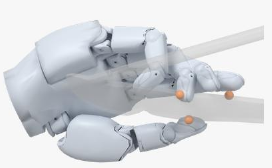
\includegraphics[width=.235\columnwidth]{figs/gesture_hanger_wuji.png} &
        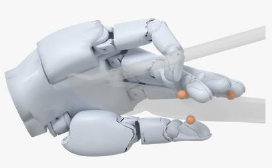
\includegraphics[width=.235\columnwidth]{figs/gesture_hanger_geort.png} &
        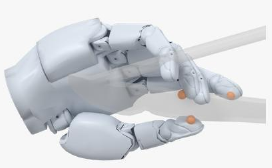
\includegraphics[width=.235\columnwidth]{figs/gesture_hanger_card.png} &
        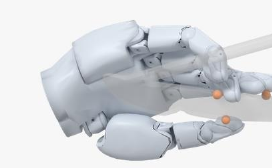
\includegraphics[width=.235\columnwidth]{figs/gesture_hanger_cart.png} \\[1pt]
        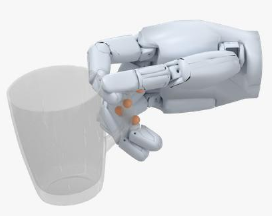
\includegraphics[width=.235\columnwidth]{figs/gesture_wuji.png} &
        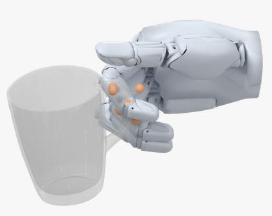
\includegraphics[width=.235\columnwidth]{figs/gesture_geort.png} &
        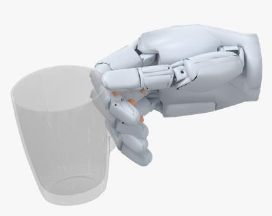
\includegraphics[width=.235\columnwidth]{figs/gesture_card.png} &
        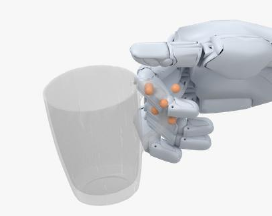
\includegraphics[width=.235\columnwidth]{figs/gesture_cart.png}
    \end{tabular}
    \caption{Example hand configurations for hanger (top) and cup (bottom) grasps. Renderings are adapted from~\cite{dai2026card}.}
    \label{fig:experiment-gestures}
\end{figure}

\emph{Draft analysis pending measurement.} We expect similar success rates for thumb-to-finger pinches across the four methods because their objectives encourage fingertip closure. For grasps with measured tactile contact, we expect wuji-retargeting and GeoRT to leave larger gaps between active taxels and the corresponding robot surfaces, especially on large objects. These gaps indicate that the robot missed contacts measured by the glove. A plausible explanation is that kinematic retargeting favors fingertip proximity in pinches and bone-direction alignment in open-hand poses. A wide grasp can therefore match the demonstrated finger directions while leaving a gap at the intended contacts. We expect CARD and CART to reduce these gaps. For continuous motion, we expect CART to require less planning time than CARD and achieve a higher smooth rate and better contact retention on the same link (Table~\ref{tab:experiment-sim}).

\subsection{Real-Robot Manipulation}
\label{sec:experiment-real}

We retarget manipulation at 1:1 physical scale with matching objects on the human and robot sides. The tasks are flower arrangement, plush-toy pickup, cup stacking, phone pickup, pen pickup and writing, and pen spinning. In the offline condition, all methods retarget the same recorded demonstrations for robot replay. In the online condition, the robot follows a live demonstration (Fig.~\ref{fig:experiment-real-frames}). For CART, the operator's observation stream leads robot-side execution by ten frames. When the robot updates from frame $t$, the synchronized EMF poses and tactile arrays through frame $t+10$ are already buffered. For each task, the operator follows a fixed gesture sequence without adapting it to the method or the robot's behavior.

Success rate is the fraction of trials in which the robot completes the entire task. Contact stability is the fraction of required link--frame contacts that the corresponding robot link maintains. The contact point may move along that link. We apply the same smooth-rate and planning-time definitions as in simulation. Table~\ref{tab:experiment-real} reports the four metrics separately for offline and online execution.

\emph{Draft analysis pending measurement.} We expect CART to achieve the highest task success rate in Table~\ref{tab:experiment-real}. We anticipate that wuji-retargeting will fail on nearly all large-object grasps, such as picking up the vase or phone, with similar failures for GeoRT. CARD's longer planning time can make online motion visibly lag, and intermittent contact loss can cause the robot to drop an object during transport after a successful pickup. We expect less visible lag with CART during live execution. This visual comparison includes buffering and robot response, whereas the reported planning time measures computation alone. We expect CART's smoother trajectories and more persistent link contact to contribute to its higher success rate.

\begin{figure*}[!t]
    \centering
    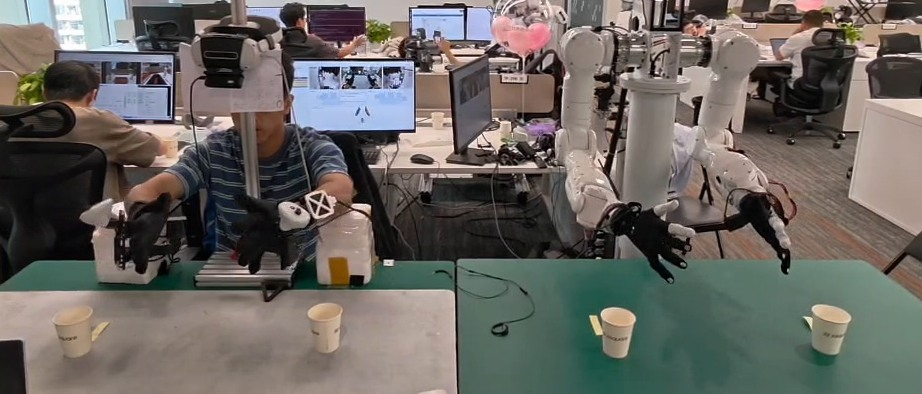
\includegraphics[width=.326\textwidth]{figs/real_robot_frame_1.jpg}\hfill
    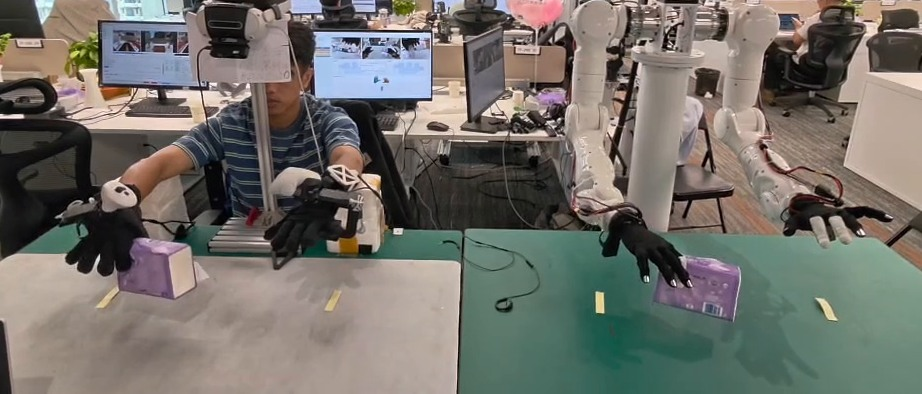
\includegraphics[width=.326\textwidth]{figs/real_robot_frame_3.jpg}\hfill
    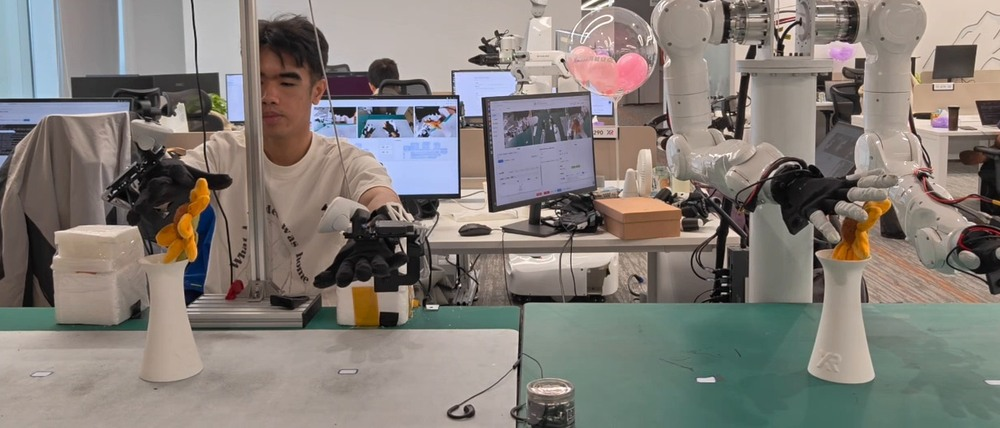
\includegraphics[width=.326\textwidth]{figs/real_robot_frame_9.jpg}\\[2pt]
    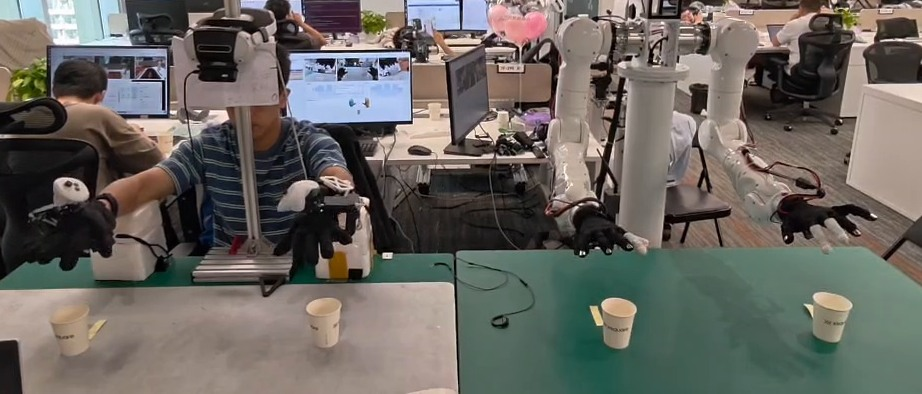
\includegraphics[width=.326\textwidth]{figs/real_robot_frame_7.jpg}\hfill
    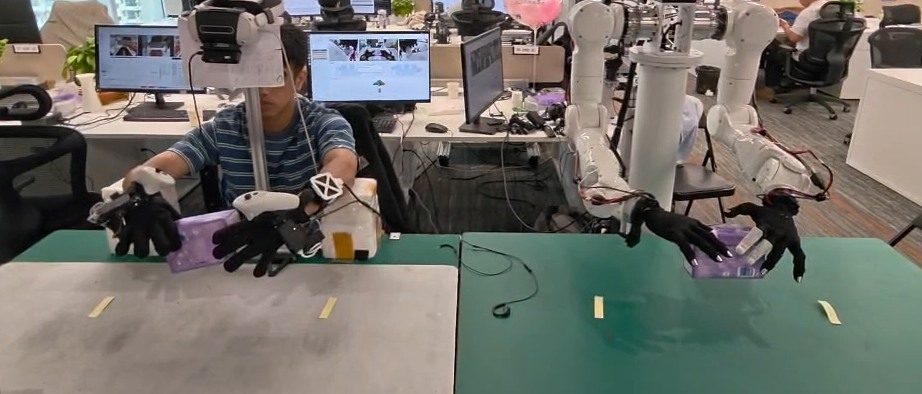
\includegraphics[width=.326\textwidth]{figs/real_robot_frame_8.jpg}\hfill
    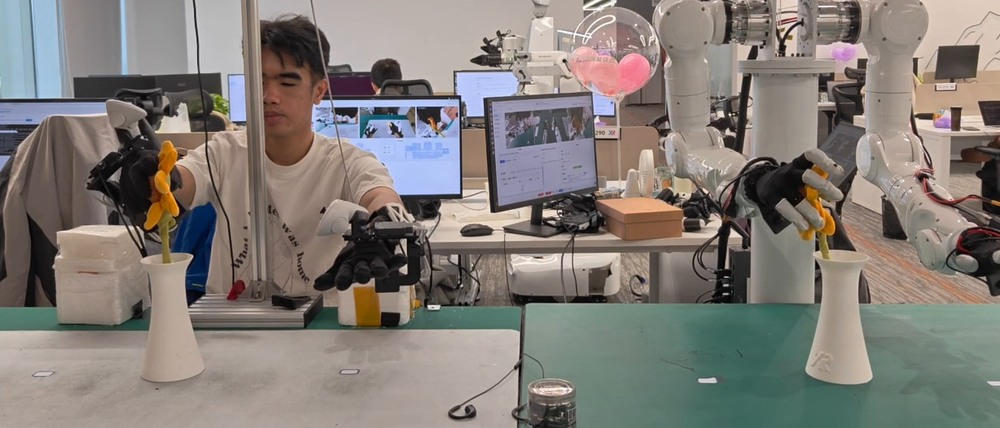
\includegraphics[width=.326\textwidth]{figs/real_robot_frame_5.jpg}\\[2pt]
    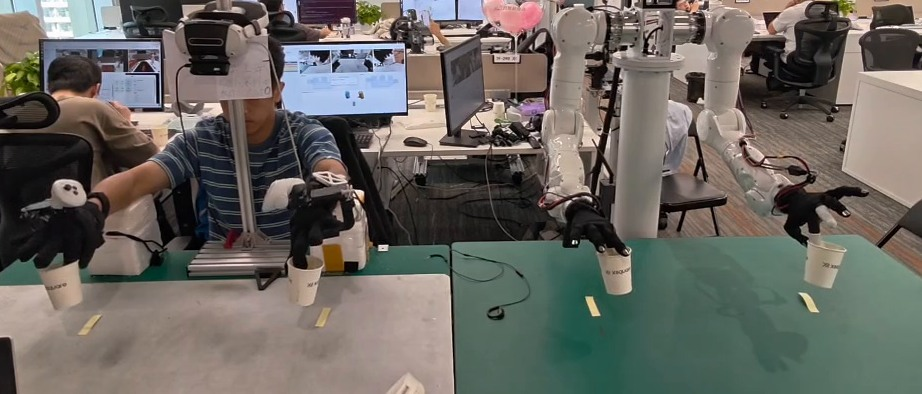
\includegraphics[width=.326\textwidth]{figs/real_robot_frame_2.jpg}\hfill
    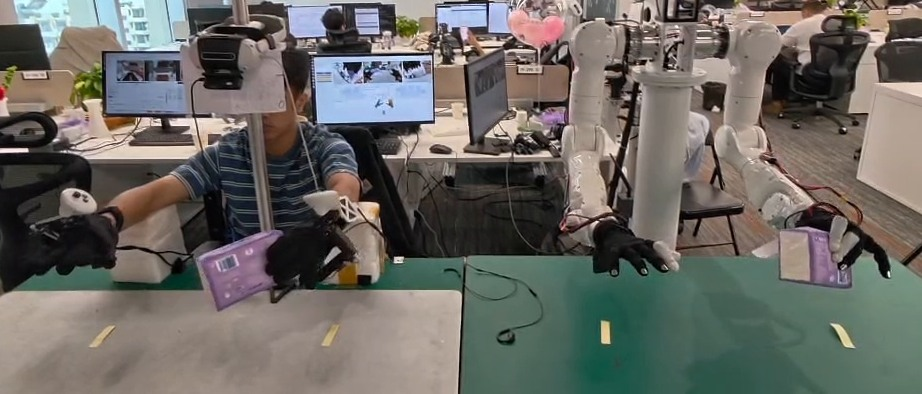
\includegraphics[width=.326\textwidth]{figs/real_robot_frame_4.jpg}\hfill
    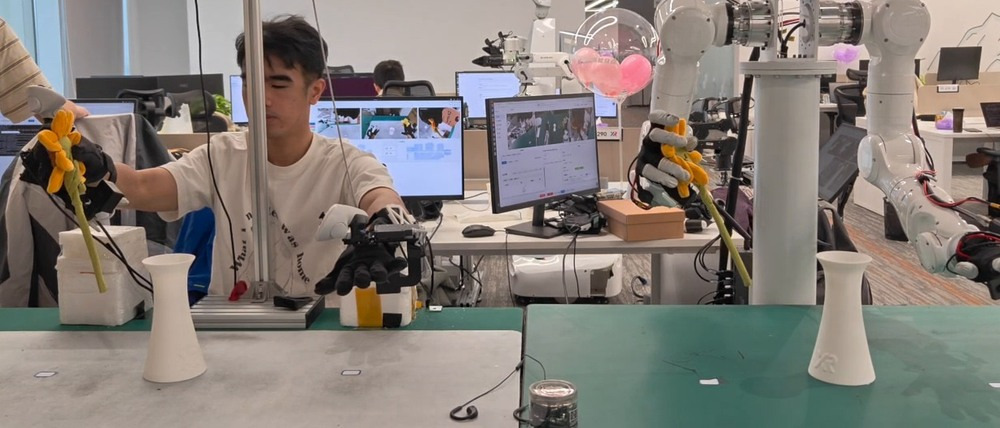
\includegraphics[width=.326\textwidth]{figs/real_robot_frame_6.jpg}
    \caption{Frames from online real-robot retargeting. Columns show cup, box, and flower handling. Rows show three stages in chronological order. The operator is on the left of each frame and the robot is on the right.}
    \label{fig:experiment-real-frames}
\end{figure*}

\subsection{Nonprehensile Manipulation}
\label{sec:experiment-nonprehensile}

We evaluate contact transfer during pen spinning, Rubik's Cube turning, and card extraction. These tasks require the fingers to release, slide, or re-establish contact as the object moves. A trial succeeds when the robot completes the prescribed pen rotation, turns the designated cube layer, or extracts the target card. We assess contact stability on the links required at each stage of the demonstration and allow the contact points to move along those links.

% !TeX root = main.tex
\section{Conclusion}
\label{sec:conclusion}

% The qualitative baseline comparison follows the author-provided results summary.
% Fill and verify the pending experimental tables before final submission.
In this work, we propose CART, a real-time retargeting method that enables a dexterous robot hand to replay human manipulation. Whereas kinematic retargeting primarily seeks postural similarity, CART uses tactile observations to represent task-relevant contacts and trains a network to preserve them across hand embodiments. Pretrained differentiable contact and collision geometry supplies trajectory-level cost gradients for policy optimization using standard BPTT. The network is trained using approximately 5~min of recorded gestures and real-world manipulation data. Each update requires a single forward pass, supporting buffered online execution. Experiments across prehensile and nonprehensile manipulation tasks show higher success rates and retargeting update rates, more stable contacts, and smoother trajectories than the evaluated baselines. These capabilities support high-quality processing of egocentric manipulation demonstrations, real-time data collection, and dexterous teleoperation.

\begin{samepage}
\textit{Limitations and future work.} Although CART supports real-time, contact-feasible retargeting, its tactile representation omits explicit object state and does not support task-level closed-loop correction. Its lightweight network is designed for retargeting and cannot serve as a standalone System~0 manipulation controller. CART also lacks zero-shot transfer across operators with different hand sizes, requiring retraining for each user despite the modest training cost. Future work could incorporate additional sensing modalities for object-aware feedback and develop a more general network that transfers across human operators.

\end{samepage}


\bibliographystyle{IEEEtran}
\bibliography{reference}

\end{document}
